\documentclass[acmsmall,review,screen]{acmart}

%% TODO during camera-ready
%% copyright
\setcopyright{acmcopyright}
\copyrightyear{2024}
\acmYear{2024}
\acmDOI{XXXXXXX.XXXXXXX}

%% conference information
\acmConference[PLDI'24]{Make sure to enter the correct conference title from
your rights confirmation emai}{June 03--05, 2018}{Woodstock, NY}
\acmPrice{15.00}
\acmISBN{978-1-4503-XXXX-X/18/06}

%% macros with packages
% load packages
\usepackage{float}
\usepackage{amsmath,amsfonts}
\usepackage{algpseudocode}
\usepackage[ruled, vlined,linesnumbered]{algorithm2e}
\usepackage{graphicx}
\usepackage{textcomp}
\usepackage{xcolor}
\usepackage{soul}
\usepackage{listings}
\usepackage{caption}
\usepackage{subcaption}
\usepackage{multirow}
\usepackage{booktabs}
\usepackage{makecell}
\usepackage{galois}
\usepackage{mathpartir}
\usepackage{bussproofs}
\usepackage{mathtools}
\usepackage{colortbl}
\usepackage{hhline}
\usepackage{stmaryrd}
\usepackage{microtype}
\usepackage{hyperref}
\usepackage{balance}
\usepackage{adjustbox}
\usepackage{tikz}
\usepackage{csquotes}
\usepackage{url}
\usepackage{amstext} % for \text macro
\usepackage{array}   % for \newcolumntype macro

% box
\newcommand{\cfbox}[2]{%
  \colorlet{currentcolor}{.}%
  {\color{#1}%
  \fbox{\color{currentcolor}#2}}%
}
\newcommand{\lcolorbox}[2]{\adjustbox{padding=0ex 1ex 1ex 1ex, bgcolor=#1}{#2}}
\newcommand{\rcolorbox}[2]{\adjustbox{padding=1ex 1ex 0ex 1ex, bgcolor=#1}{#2}}

% table rules
\newcolumntype{?}{!{\vrule width 1pt}}
\newcommand*{\belowrulesepcolor}[1]{%
  \noalign{%
    \kern-\belowrulesep
    \begingroup
      \color{#1}%
      \hrule height\belowrulesep
    \endgroup
  }%
}
\newcommand*{\aboverulesepcolor}[1]{%
  \noalign{%
    \begingroup
      \color{#1}%
      \hrule height\aboverulesep
    \endgroup
    \kern-\aboverulesep
  }%
}

% colors
\definecolor{gainsboro}{rgb}{0.86, 0.86, 0.86}
\definecolor{dkgreen}{rgb}{0, 0.5, 0}
\definecolor{lightred}{rgb}{0.93, 0.57 0.52}
\definecolor{esnt}{rgb}{0.20, 0.20, 0.20}
\definecolor{esparam}{rgb}{0.16, 0.63, 0.59}
\definecolor{esalg}{rgb}{0.12, 0.42, 0.65}
\definecolor{esvar}{rgb}{0.16, 0.63, 0.59}
\definecolor{gray1}{rgb}{0.95, 0.95, 0.95}
\definecolor{gray2}{rgb}{0.85, 0.85, 0.85}
\definecolor{gray3}{rgb}{0.75, 0.75, 0.75}

\newcolumntype{L}{>{$}l<{$}} % math-mode version of "l" column type
\newcommand{\llb}{\llbracket}
\newcommand{\rrb}{\rrbracket}

% basic
\newcommand*{\sphinxDeclareColorOption}[2]{%
   \definecolor{#1}#2%
}%
\sphinxDeclareColorOption{InnerLinkColor}{{rgb}{0.208,0.374,0.486}}
\newcommand{\inblue}[1]{{\color{InnerLinkColor}{#1}}}
%\newcommand{\inblue}[1]{{\color{blue}{#1}}}
\newcommand{\inred}[1]{{\color{red}{#1}}}
\newcommand{\x}[1]{\inred{#1}}
\newcommand{\y}[1]{\textbf{\inred{#1}}}
\newcommand{\todo}{\inred{TODO}}
%\newcommand{\powerset}{\mathcal{P}}
\newcommand{\tif}{\text{if} \; }
\newcommand{\telse}{\text{otherwise}}
\newcommand{\tst}{{\; \text{s.t.} \; }}

% Our tool name
\newcommand{\name}[1]{\textsf{#1}\xspace}
\newcommand{\ssf}[1]{\ensuremath{\mathsf{#1}}\xspace}
\newcommand{\sbf}[1]{\textbf{\small #1}\xspace}
\newcommand{\stt}[1]{\texttt{\small #1}\xspace}
\newcommand{\dsl}{\name{Wasm-DSL}}
\newcommand{\dl}{\name{DL}}
\newcommand{\al}{\name{AL}}
\newcommand{\spectec}{\name{\$SRC}}
\newcommand{\dslname}{SpecTec\xspace}
\newcommand{\ires}{\ssf{IR_{\mathsf{ES}}}}

% codes
\newcommand{\code}[1]{\text{\lstinline[style=JS]!#1!}} 
\newcommand{\scode}[1]{\texttt{\scriptsize #1}} 
\newcommand{\bcode}[1]{\texttt{\small #1}}
\newcommand{\ircode}[1]{\text{\lstinline[style=ires]!#1!}}

\newcommand{\kwsyn}{\bcode{syntax}}
\newcommand{\kwret}{\bcode{return}}

\newcommand{\kwalg}{\bcode{algorithm}}
\newcommand{\kweq}{\coloneqq}
\newcommand{\kwdef}{\bcode{def}}
\newcommand{\kwif}{\bcode{if}}
\newcommand{\kwreturn}{\bcode{return}}
\newcommand{\kweither}{\bcode{either}}
\newcommand{\kwenter}{\bcode{enter}}
\newcommand{\kwassert}{\bcode{assert}}
\newcommand{\kwpush}{\bcode{push}}
\newcommand{\kwpop}{\bcode{pop}}
\newcommand{\kwpopall}{\bcode{popall}}
\newcommand{\kwlet}{\bcode{let}}
\newcommand{\kwtrap}{\bcode{trap}}
\newcommand{\kwnop}{\bcode{nop}}
\newcommand{\kwexecute}{\bcode{execute}}
\newcommand{\kwexecuteseq}{\bcode{executeseq}}
\newcommand{\kwperform}{\bcode{perform}}
\newcommand{\kwexit}{\bcode{exit}}
\newcommand{\kwref}{\bcode{ref}}
\newcommand{\kwreplace}{\bcode{replace}}
\newcommand{\kwiscaseof}{\bcode{iscaseof}}
\newcommand{\kwisdefined}{\bcode{isdefined}}
\newcommand{\kwisvalid}{\bcode{isvalid}}
%\newcommand{\kwwasmc}{\bcode{wasmc}}
%\newcommand{\kw}{\bcode{}}
\newcommand{\kwnot}{\bcode{not}}
\newcommand{\kwequ}{\bcode{=}}
\newcommand{\kwrl}{\bcode{(}}
\newcommand{\kwrr}{\bcode{)}}
\newcommand{\kwcl}{\bcode{\{}}
\newcommand{\kwcr}{\bcode{\}}}
\newcommand{\kwsl}{\bcode{[}}
\newcommand{\kwsr}{\bcode{]}}
\newcommand{\kwass}{\bcode{:=}}
\newcommand{\kwext}{\bcode{:+}}
\newcommand{\kwcat}{\bcode{++}}

\newcommand{\unop}{\ensuremath{\otimes}}
\newcommand{\binop}{\ensuremath{\oplus}}

% Basic
\DeclareMathAlphabet{\mathpzc}{T1}{pzc}{m}{it}
\newcommand{\powerset}[1]{\mathcal{P}(#1)}
\newcommand{\abs}[1]{\widehat{#1}}
\newcommand{\finmap}{{\xrightarrow[]{\text{fin}}}}
\newcommand{\mapstos}{\;\dot{\mapsto}\;}
\newcommand{\Dom}{\name{Dom}}
\DeclarePairedDelimiter{\norm}{\lvert}{\rvert} 

% JavaScript
\newcommand{\js}{\name{js}}

% Getters
\newcommand{\getfunc}{\name{func}}
\newcommand{\getinst}{\name{inst}}
\newcommand{\getnext}{\name{next}}
\newcommand{\getcaller}{\name{caller}}
\newcommand{\getlab}{\name{label}}

% Values
\newcommand{\valset}{\mathbb{V}}
\newcommand{\val}{v}
\newcommand{\pvalset}{\valset^\name{p}}
\newcommand{\pval}{\val^\name{p}}
\newcommand{\boolset}{\valset_\name{bool}}
\newcommand{\bool}{b}
\newcommand{\true}{\code{\#t}}
\newcommand{\false}{\code{\#f}}
\newcommand{\intset}{\valset_\name{int}}
\newcommand{\strset}{\valset_\name{str}}

% JavaScript ASTs
\newcommand{\treeset}{\mathbb{T}}
\newcommand{\tree}{t}
\newcommand{\trees}{\overline{t}}
\newcommand{\nodeset}{\Phi}
\newcommand{\node}{\phi}
\newcommand{\subtree}{\lhd}
\newcommand{\getsubs}{\name{subs}}
\newcommand{\treetop}{\code{\#}}
\newcommand{\ty}{\tau}
\newcommand{\eval}{\code{eval}}

% DL Syntax
\newcommand{\defnset}{\mathfrak{D}}
\newcommand{\defn}{d}
\newcommand{\infrset}{\mathcal{R}}
\newcommand{\infr}{r}
\newcommand{\funcset}{\mathcal{F}}
\newcommand{\func}{f}

% AL Syntax
\newcommand{\progset}{\mathfrak{P}}
\newcommand{\prog}{p}
\newcommand{\algset}{\mathcal{A}}
\newcommand{\alg}{a}
\newcommand{\instset}{\mathcal{I}}
\newcommand{\inst}{i}
\newcommand{\exprset}{\mathcal{E}}
\newcommand{\expr}{e}
\newcommand{\condset}{\mathcal{C}}
\newcommand{\cond}{c}
\newcommand{\numset}{\mathcal{N}}
\newcommand{\num}{n}
\newcommand{\qualset}{\mathcal{Q}}
\newcommand{\qual}{q}
\newcommand{\wasmcset}{\mathcal{W}}
\newcommand{\wasmc}{w}
\newcommand{\cnstrset}{\mathcal{K}}
\newcommand{\cnstr}{k}

% Variables
\newcommand{\varset}{\mathcal{X}}
\newcommand{\varx}{x}
\newcommand{\varf}{f}
\newcommand{\vart}{t}
\newcommand{\varp}{p}

% Field Mappings
\newcommand{\fmapset}{\mathbb{M}}
\newcommand{\fmap}{m}
\newcommand{\jsfmapset}{\fmapset_\js}
\newcommand{\jsfmap}{\fmap_\js}

% Transition Relations
\newcommand{\trans}[1]{\leadsto_{#1}}

\newcommand{\hide}[1]{}
\newcommand{\unify}{\ensuremath{\mathcal{U}}\xspace}
\newcommand{\dltoil}{\ensuremath{\mathcal{T}}\xspace}


%% start document
\begin{document}

%% title information
\title{
SpecTec: Bridging the Gap between Declarative and Algorithmic Semantics
}

\author{Anonymous Author(s)}

%% authors
%
% \author{Dongjun Youn}
% \email{f52985@kaist.ac.kr}
% \orcid{0000-0002-5766-2035}
% \affiliation{%
%   \institution{KAIST}
%   \city{Daejeon}
%   \country{South Korea}
% }
%
% \author{Wonho Shin}
% \email{???@kaist.ac.kr}
% \orcid{????-????-???-????}
% \affiliation{%
%   \institution{KAIST}
%   \city{Daejeon}
%   \country{South Korea}
% }
% \author{Jaehyun Lee}
% \email{???@kaist.ac.kr}
% \orcid{????-????-????-????}
% \affiliation{%
%   \institution{KAIST}
%   \city{Daejeon}
%   \country{South Korea}
% }
%
% \author{Sukyoung Ryu}
% \email{sryu.cs@kaist.ac.kr}
% \orcid{0000-0002-0019-9772}
% \affiliation{%
%   \institution{KAIST}
%   \city{Daejeon}
%   \country{South Korea}
% }

%% abstract

%% TODO http://dl.acm.org/ccs.cfm during camera ready
% \begin{CCSXML}
% <ccs2012>
%  <concept>
%   <concept_id>10010520.10010553.10010562</concept_id>
%   <concept_desc>Computer systems organization~Embedded systems</concept_desc>
%   <concept_significance>500</concept_significance>
%  </concept>
%  <concept>
%   <concept_id>10010520.10010575.10010755</concept_id>
%   <concept_desc>Computer systems organization~Redundancy</concept_desc>
%   <concept_significance>300</concept_significance>
%  </concept>
%  <concept>
%   <concept_id>10010520.10010553.10010554</concept_id>
%   <concept_desc>Computer systems organization~Robotics</concept_desc>
%   <concept_significance>100</concept_significance>
%  </concept>
%  <concept>
%   <concept_id>10003033.10003083.10003095</concept_id>
%   <concept_desc>Networks~Network reliability</concept_desc>
%   <concept_significance>100</concept_significance>
%  </concept>
% </ccs2012>
% \end{CCSXML}
%
% \ccsdesc[500]{Computer systems organization~Embedded systems}
% \ccsdesc[300]{Computer systems organization~Redundancy}
% \ccsdesc{Computer systems organization~Robotics}
% \ccsdesc[100]{Networks~Network reliability}
\keywords{
  WebAssembly,
  language specification,
  executable prose,
  DSL,
}

\maketitle

%% body of the paper
\section{Introduction}\label{sec:intro}
\begin{figure}[t]
  \centering
  \begin{subfigure}{\textwidth}
    \centering
    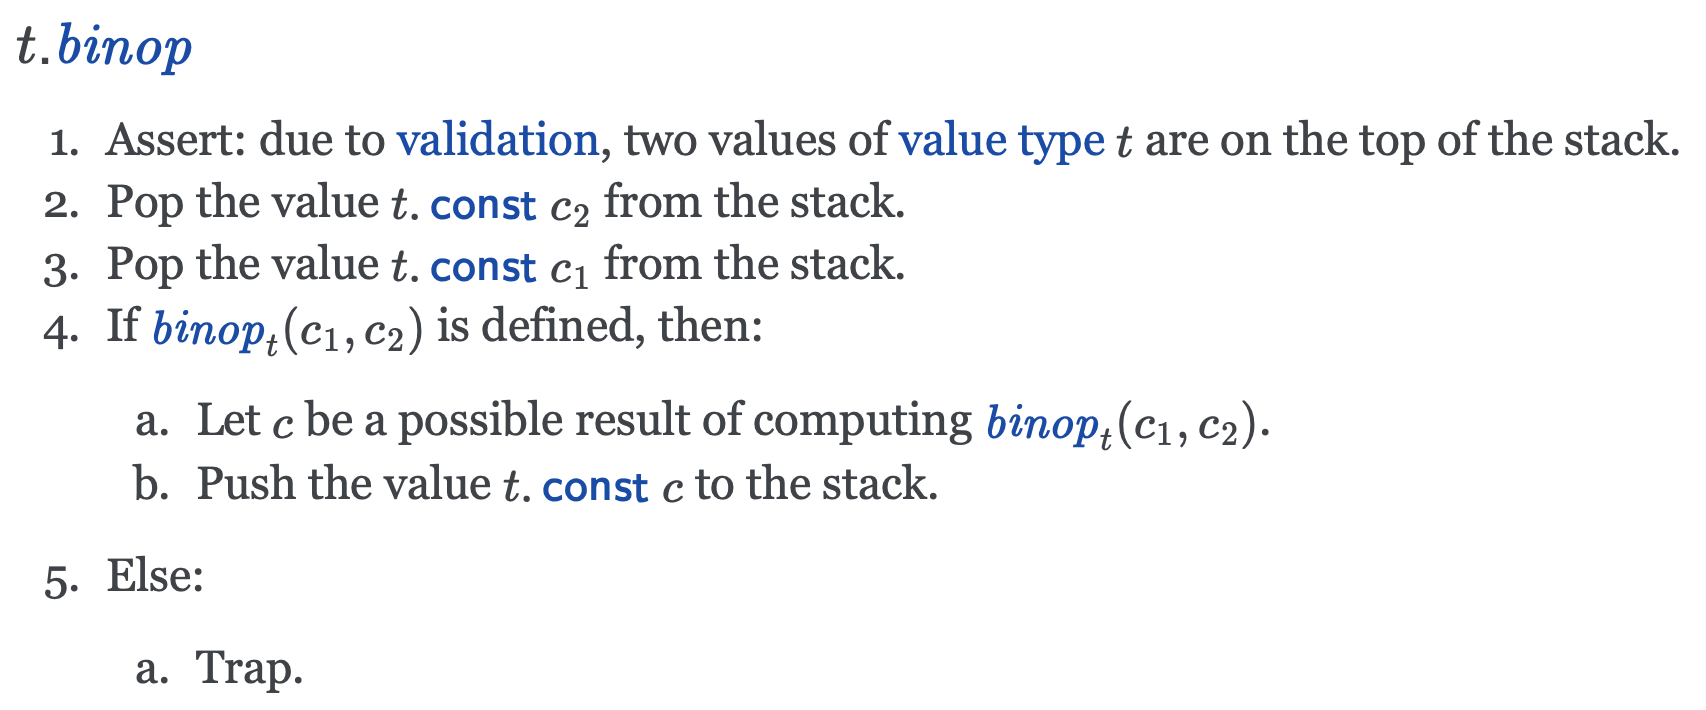
\includegraphics[width=.7\textwidth]{../img/spec-prose.png}
\vspace*{-1em}
    \subcaption{Prose notation}
\vspace*{.5em}
  \end{subfigure}
  \begin{subfigure}{\textwidth}
    \centering
    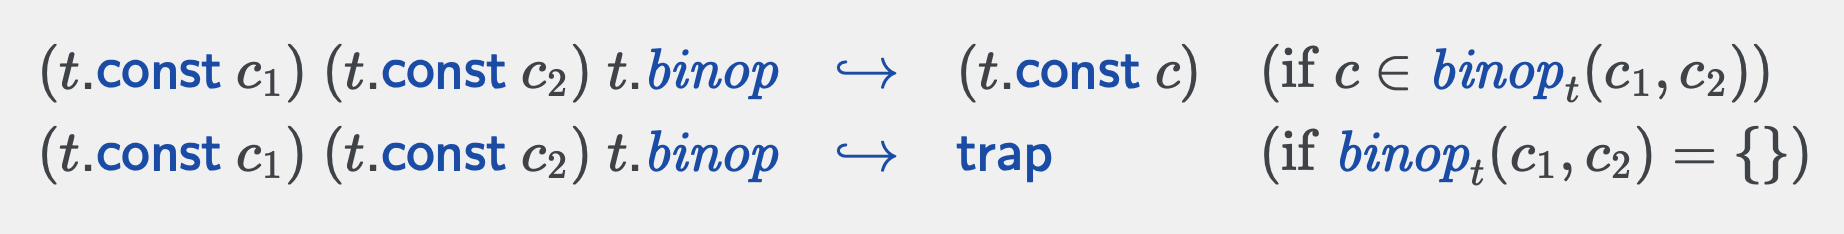
\includegraphics[width=.7\textwidth]{../img/spec-formal.png}
    \subcaption{Formal notation}
  \end{subfigure}
\caption{Semantics of \ensuremath{t.\mathit{\inblue{binop}}} in the specification}
\label{fig:spec}
\end{figure}

A programming language is defined by its syntax and semantics.
Syntax and semantics are the basis for all subsequent development and
analysis of the language, so it is important to define them clearly and rigorously. 
Many programming languages, such as Java~\cite{javaspec} and Python~\cite{pythonspec},
therefore have language specifications that define their syntax and semantics.
For languages that are prone to implementation inconsistency issues,
such as C~\cite{cstandard} and JavaScript~\cite{ecmascript},
international committees define them according to their own standardization processes.
Some languages, like Standard ML~\cite{sml}, even have formal descriptions
that define them in mathematical notation.

WebAssembly (Wasm) is a low-level bytecode language and virtual machine~\cite{wasmspec}.
It was initially designed as an efficient compilation target and execution model on Web platforms
and has been adopted across a wide range of ecosystems,
including cloud and edge computing~\cite{lucet, cloudflare}, 
mobile and embedded systems~\cite{wasm-embedded}, IoT~\cite{wasm-iot}, and
blockchains~\cite{wasm-blockchain}.
Because different browsers implement Wasm within vendor-specific architectures
using multi-tier interpretation or just-in-time compilation,
Wasm faces the risk of implementation discrepancies.
The diversity of the various ecosystems exacerbates the situation.

To mitigate these risks, Wasm has been standardized by
the W3C Wasm Community Group~\cite{wasm-w3c}.
It requires four key artifacts for a feature to be standardized:
1) a \textit{formal specification} for the feature in declarative-style rewrite rules, written in LaTeX;
2) a \textit{prose pseudocode} presenting an algorithmic-style semantics, written in reStructuredText markup;
3) an extended \textit{reference interpreter} with the implementation of the feature, written in OCaml; and
4) a \textit{unit test suite} for the feature, written in the Wasm text format.
All of these artifacts must define the same behavior of a Wasm program.
Note that the specification provides \textit{both} declarative and algorithmic styles of semantic definitions.
For example, Fig.~\ref{fig:spec} shows the execution semantics of the binary operation instruction
$t.\mathit{\inblue{binop}}$ in the official Wasm specification.
Fig.~\ref{fig:spec}(a) presents the semantics in a prose notation broken down into five steps,
while Fig.~\ref{fig:spec}(b) specifies it in a formal notation using rewrite rules.

The two styles of semantic definitions cater to the dual needs of
language ``designers'' and ``implementers.''  Declarative rewrite
rules serve the needs of designers by focusing on clarity and
correctness of language semantics. They allow theorem provers like
Coq, Isabelle, Lean, and Agda to mechanize language semantics
and prove various properties, including type safety.
Algorithmic prose pseudocode, on the other hand, helps implementers
understand language behavior. A step-by-step description of the
language semantics can be a good guide to how to implement it.

Despite the onerous standardization process, the Wasm specification has been
written and maintained \textit{manually}, which creates challenges for specification writers.
Writing the prose is extremely laborious~\cite{Andreasicfp23}, and code reviews of
feature proposals written in LaTeX and reStructuredText are not user-friendly.
Manual processes are vulnerable to human error, potentially leading
to inconsistencies or inaccuracies in the specification.
As Wasm grows with new language features such as Garbage Collected Types, Threads,
and Exception Handling that will be supported by Wasm 3.0,
manually crafting all of the artifacts is not scalable.

These challenges call for the need to automate the process or \textit{mechanize} the language semantics.
For declarative-style rewrite rules, the literature shows general-purpose language frameworks such as
Ott~\cite{ott}, PLTRedex~\cite{pltredex}, Skeleton~\cite{skeleton}, Spoofax~\cite{spoofax},
and the K framework~\cite{k}. Among them, the K framework can generate various tools,
including interpreters, model checkers, and verifiers, from a language specification written in its language K.
It has specified the core semantics of real-world programming languages
such as C~\cite{kc}, Java~\cite{kjava}, Python~\cite{kpython}, and JavaScript~\cite{kjs}.
For algorithmic-style semantics, the ESMeta framework~\cite{esmeta}
can extract a mechanized specification from
an ECMAScript/JavaScript specification~\cite{ecmascript} and automatically
generate diverse tools~\cite{jiset,jest,jstar,jsaver}.
%
%  ESMeta parses the structured English prose algorithms of ECMAScript
% Specification document, and translates them into an internal representation, $IR_{ES}$.
%   $IR_{ES}$ has its own semantics, and thus can be executed with an interpreter implementation.
%   Executing the JavaScript semantics written in $IR_{ES}$ allows an indirect execution of JavaScript programs.
%   Utilizing the executable semantics, ESMeta derives a type checker for the specification, test
% suite synthesizers, and a static analyzer of JavaScript.
%
% Now, each ECMA-262 PR will execute the ESMeta type checker, and any new or changed tests in a Test262 PR will be executed using the ESMeta interpreter.
%
ESMeta has been officially integrated into the continuous integration (CI) systems of
the ECMAScript specification~\cite{ciecma262} and the Test262 conformance test suite~\cite{citest262}
since November 2022.
Because the existing language frameworks can mechanize only one style of semantics,
they are not applicable to Wasm, which should support both declarative and algorithmic styles of semantics.

\begin{figure}[t]
\footnotesize
\begin{verbatim}
                rule Step_pure/binop-val:
                    (CONST nt c_1) (CONST nt c_2) (BINOP nt binop) ~> (CONST nt c)
                    -- if $binop(binop, nt, c_1, c_2) = c

                rule Step_pure/binop-trap:
                    (CONST nt c_1) (CONST nt c_2) (BINOP nt binop) ~> TRAP
                    -- if $binop(binop, nt, c_1, c_2) = epsilon
\end{verbatim}
\caption{The binary operator semantics in \spectec's DSL}
\label{fig:dsl}
\end{figure}

In this paper, we propose \spectec, a framework for mechanizing Wasm semantics in both styles.
\spectec presents a \emph{Domain-Specific Language (DSL)} that
defines the Wasm syntax, type system, and execution semantics in a declarative style,
which serves as a single source of truth.
Figure~\ref{fig:dsl} illustrates the semantics of $t.\mathit{\inblue{binop}}$ in the DSL,
which looks similar to the one in the official specification in Figure~\ref{fig:spec}(b).
Once the Wasm formal semantics is written in the DSL,
a number of tools can be automatically generated as backends:
1) declarative backends, including LaTeX-based formal specifications and
mechanized definitions in various theorem provers, and
2) algorithmic backends, such as prose specifications in reStructuredText and Wasm interpreters.
By conducting meta-level error checking and automatically generating the required specification artifacts,
\spectec can alleviate the burden on language designers and implementers.

\spectec's DSL is designed to provide a close and easy representation and reasoning of
the Wasm semantics in declarative backends.
It can directly produce LaTeX-based formal specifications from the definitions in the DSL,
and all definitions and variables in the DSL are ``type-checked'' to detect ill-formed ones.
It can also generate mechanized definitions for theorem provers.
This saves language designers the trouble of manually specifying
language semantics in different theorem provers every time the specification is updated.

On the contrary, algorithmic backends are not directly produced from the definitions in the DSL,
but from the definitions in the \emph{Algorithmic Language (AL)}.
The AL is designed to provide a close and easy representation and manipulation of
the Wasm semantics in the official prose specification,
so the English prose in reStructuredText markup can be generated directly from the definitions in the AL.
\spectec can also support the interpretation of Wasm programs,
following the approach of the ESMeta framework.

To bridge the gap between the two styles of semantics,
we present a mechanism for automatically deriving algorithmic ALs from declarative DSLs.
Several challenges arise in transforming declarative-style rewrite rules
into algorithmic-style prose pseudocode.
For example, a single Wasm instruction may have multiple rewrite rules,
each expressing certain premises,
but each instruction should have only one prose pseudocode. 
In addition, the equals operator `$=$' in mathematical rules
can be ambiguous, as it can mean assignment or equality checking.
We show that the transformation is an NP-hard problem
and propose a practical solution.

\spectec is available as an open-source project~\cite{spectec}
and covers everything in Wasm 2.0 except SIMD instructions.
The automatically generated Wasm semantics in the AL passes
100\% of the official test suite (except for SIMD) using an AL interpreter.
To further specify the semantics for Wasm 3.0, we only needed
to make minor adjustments in \spectec. During this process, we
reported a few errors in the Garbage Collected Types proposal and
received confirmation from the proposal champions.

This paper presents the following contributions:
\begin{itemize}
\item \textbf{\spectec is the first language semantics framework that
embraces both declarative and algorithmic styles of semantics.}
Unlike existing language frameworks that can mechanize only one style of semantics,
\spectec can support both styles of semantics.

\item \textbf{\spectec can automatically generate multiple backends from 
a single source of truth.}
It is designed to be easy to write, read, and reivew, enabling
meta-level error detection in the Wasm specification.

\item \textbf{\spectec is a forward-compatible toolchain that can
adapt to the evolving Wasm semantics.}
To evaluate \spectec's forward compatibility, we applied it to five
proposals in Wasm 3.0 and found that only minor adjustments were necessary. 
\end{itemize}


%% TODO during the camera ready
%% acknowledgements
% \begin{acks}
% This work was supported by National Research Foundation of
% Korea (NRF) (Grants NRF-2017R1A2B3012020 and 2017M3C4A7068177).

%% bibliography style
\bibliographystyle{ACM-Reference-Format}

%% the bibliography file.
\balance
\bibliography{ref}

\end{document}
\endinput
